\documentclass[tikz,border=1pt]{standalone}
\usepackage{lmodern}\renewcommand{\familydefault}{\sfdefault}\usepackage[T1]{fontenc}
\usetikzlibrary{arrows.meta,positioning,calc}
\definecolor{ink}{HTML}{1A1A1A}\definecolor{gr}{HTML}{8A8A8A}\definecolor{grf}{HTML}{F2F2F2}
\definecolor{or}{HTML}{D55E00}\definecolor{orf}{HTML}{FDEEE6}\definecolor{gn}{HTML}{009E73}\definecolor{gnf}{HTML}{E6F5F0}
\definecolor{bl}{HTML}{0072B2}\definecolor{blf}{HTML}{E6F1F9}\definecolor{panel}{HTML}{FAFAFA}\definecolor{pline}{HTML}{C8C8C8}
\definecolor{bl}{HTML}{0072B2}\definecolor{blf}{HTML}{E6F1F9}
\tikzset{
  box/.style={draw=gr,fill=grf,line width=0.6pt,rounded corners=2pt,minimum width=2.3cm,minimum height=0.9cm,text width=2.15cm,align=center,inner sep=2pt,font=\footnotesize,text=ink},
  mukv/.style={box,draw=or,fill=orf,line width=0.8pt},
  outc/.style={box,draw=gn,fill=gnf,line width=0.8pt},
  cbox/.style={draw=gr,fill=grf,line width=0.6pt,rounded corners=2pt,minimum width=2.95cm,text width=2.8cm,minimum height=1.55cm,align=center,inner sep=2pt,font=\footnotesize,text=ink},
  cmukv/.style={cbox,draw=or,fill=orf,line width=0.8pt},
  wide/.style={cbox,minimum width=7.6cm,text width=7.4cm,minimum height=1.2cm},
  wmukv/.style={wide,draw=or,fill=orf,line width=0.8pt},
  data/.style={-{Stealth[length=4pt,width=3.5pt]},line width=0.6pt,ink},
  ctrl/.style={-{Stealth[length=4pt,width=3.5pt]},line width=0.6pt,or,dashed},
  ctrlg/.style={-{Stealth[length=4pt,width=3.5pt]},line width=0.6pt,gr,dashed},
  heat/.style={-{Stealth[length=4pt,width=3.5pt]},line width=0.7pt,gr,dotted},
  meas/.style={-{Stealth[length=4pt,width=3.5pt]},line width=0.6pt,gn,dash dot},
  kv/.style={-{Stealth[length=4pt,width=3.5pt]},line width=0.6pt,bl},
  lab/.style={font=\scriptsize,inner sep=1pt,text=ink},
  stepn/.style={circle,fill=or,text=white,font=\bfseries\scriptsize,inner sep=0.5pt,minimum size=11pt},
  stepg/.style={stepn,fill=gr},
  stepr/.style={rectangle,rounded corners=3pt,fill=or,text=white,font=\bfseries\scriptsize,inner sep=1.5pt,minimum height=11pt},
  head/.style={font=\bfseries\scriptsize,inner sep=1pt}
}
\newcommand{\bx}[2]{\textbf{#1}\\[0pt]{\scriptsize #2}}
\begin{document}
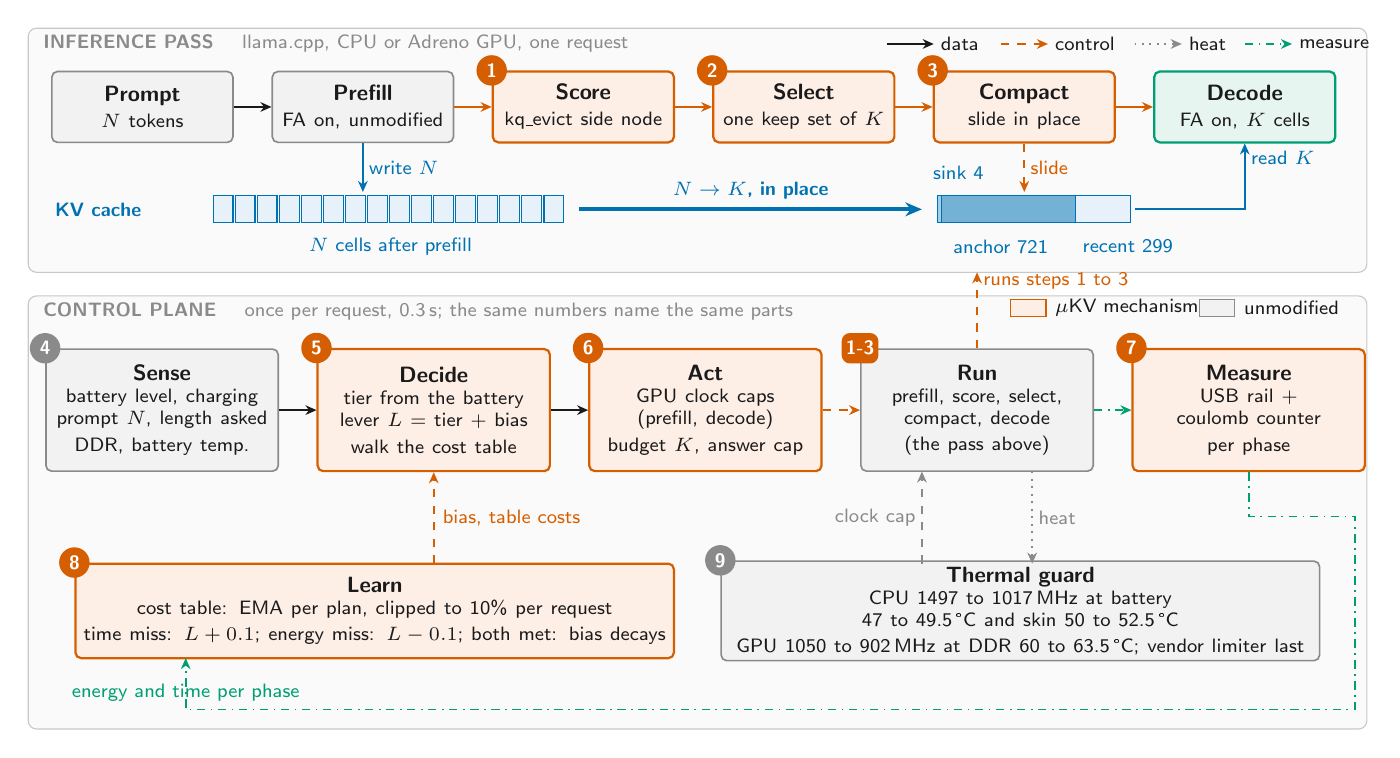
\begin{tikzpicture}[x=1cm,y=1cm]
% ===================== panel 1: the inference pass =====================
\fill[panel,draw=pline,rounded corners=3pt] (0,4.35) rectangle (17,7.45);
\node[head,anchor=north west,text=gr] at (0.15,7.4) {INFERENCE PASS \quad {\mdseries llama.cpp, CPU or Adreno GPU, one request}};
\draw[data] (10.9,7.25) -- (11.5,7.25);\node[lab,anchor=west] at (11.55,7.25) {data};
\draw[ctrl] (12.35,7.25) -- (12.95,7.25);\node[lab,anchor=west] at (13.0,7.25) {control};
\draw[heat] (14.05,7.25) -- (14.65,7.25);\node[lab,anchor=west] at (14.7,7.25) {heat};
\draw[meas] (15.45,7.25) -- (16.05,7.25);\node[lab,anchor=west] at (16.1,7.25) {measure};
% ================= the pass =================
\node[box] (prompt) at (1.45,6.45) {\bx{Prompt}{$N$ tokens}};
\node[box] (prefill) at (4.25,6.45) {\bx{Prefill}{FA on, unmodified}};
\node[mukv] (score) at (7.05,6.45) {\bx{Score}{kq\_evict side node}};
\node[mukv] (select) at (9.85,6.45) {\bx{Select}{one keep set of $K$}};
\node[mukv] (compact) at (12.65,6.45) {\bx{Compact}{slide in place}};
\node[outc] (decode) at (15.45,6.45) {\bx{Decode}{FA on, $K$ cells}};
\draw[data] (prompt) -- (prefill);
\draw[data,or] (prefill) -- (score); \draw[data,or] (score) -- (select); \draw[data,or] (select) -- (compact); \draw[data,or] (compact) -- (decode);
\node[stepn] at (score.north west) {1};\node[stepn] at (select.north west) {2};\node[stepn] at (compact.north west) {3};
% KV strip
\node[lab,text=bl,font=\bfseries\scriptsize,anchor=west] at (0.3,5.15) {KV cache};
\foreach \i in {0,...,15}{\fill[blf,draw=bl,line width=0.4pt] (2.35+\i*0.28,4.98) rectangle (2.35+\i*0.28+0.25,5.32);}
\node[lab,text=bl] at (4.6,4.68) {$N$ cells after prefill};
\draw[kv] (prefill.south) -- (4.25,5.37) node[lab,text=bl,midway,right=1pt] {write $N$};
\draw[kv,line width=1.4pt,-{Stealth[length=6pt,width=5pt]}] (7.0,5.15) -- (11.35,5.15) node[lab,text=bl,font=\bfseries\scriptsize,midway,above=2pt] {$N \to K$, in place};
% compacted strip, proportional to the measured 4 / 721 / 299 split of K = 1024
\fill[bl!35!white,draw=bl,line width=0.4pt] (11.55,4.98) rectangle (11.60,5.32);
\fill[bl!55!white,draw=bl,line width=0.4pt] (11.60,4.98) rectangle (13.30,5.32);
\fill[blf,draw=bl,line width=0.4pt] (13.30,4.98) rectangle (14.00,5.32);
\node[lab,text=bl,anchor=west] at (11.45,5.62) {sink 4};
\node[lab,text=bl] at (12.35,4.68) {anchor 721};
\node[lab,text=bl,anchor=west] at (13.35,4.68) {recent 299};
\draw[ctrl] (compact.south) -- (12.65,5.37) node[lab,text=or,midway,right=1pt] {slide};
\draw[kv] (14.05,5.15) -- (15.45,5.15) -- (decode.south) node[lab,text=bl,pos=0.78,right=1pt] {read $K$};
% ===================== panel 2: the control plane =====================
\fill[panel,draw=pline,rounded corners=3pt] (0,-1.45) rectangle (17,4.05);
\node[head,anchor=north west,text=gr] at (0.15,4.0) {CONTROL PLANE \quad {\mdseries once per request, 0.3\,s; the same numbers name the same parts}};
\node[draw=or,fill=orf,minimum width=0.45cm,minimum height=0.22cm,inner sep=0] at (12.7,3.9) {};\node[lab,anchor=west] at (13.0,3.9) {$\mu$KV mechanism};
\node[draw=gr,fill=grf,minimum width=0.45cm,minimum height=0.22cm,inner sep=0] at (15.1,3.9) {};\node[lab,anchor=west] at (15.4,3.9) {unmodified};
\node[cbox]  (sense)   at (1.7,2.60)  {\bx{Sense}{battery level, charging\\ prompt $N$, length asked\\ DDR, battery temp.}};
\node[cmukv] (decide)  at (5.15,2.60) {\bx{Decide}{tier from the battery\\ lever $L$ = tier + bias\\ walk the cost table}};
\node[cmukv] (act)     at (8.6,2.60)  {\bx{Act}{GPU clock caps\\ (prefill, decode)\\ budget $K$, answer cap}};
\node[cbox]  (run)     at (12.05,2.60){\bx{Run}{prefill, score, select,\\ compact, decode\\ (the pass above)}};
\node[cmukv] (measure) at (15.5,2.60) {\bx{Measure}{USB rail +\\ coulomb counter\\ per phase}};
\node[stepg] at (sense.north west) {4};\node[stepn] at (decide.north west) {5};\node[stepn] at (act.north west) {6};
\node[stepr] at (run.north west) {1-3};\node[stepn] at (measure.north west) {7};
\draw[data] (sense) -- (decide);
\draw[data] (decide) -- (act);
\draw[ctrl] (act) -- (run);
\draw[meas] (run) -- (measure);
\draw[ctrl] (run.north) -- (12.05,4.35) node[lab,text=or,pos=0.88,right=1pt] {runs steps 1 to 3};
\node[wmukv] (learn) at (4.4,0.05) {\bx{Learn}{cost table: EMA per plan, clipped to 10\% per request\\ time miss: $L+0.1$; energy miss: $L-0.1$; both met: bias decays}};
\node[wide]  (guard) at (12.6,0.05) {\bx{Thermal guard}{CPU 1497 to 1017\,MHz at battery 47 to 49.5\,\textdegree C and skin 50 to 52.5\,\textdegree C\\ GPU 1050 to 902\,MHz at DDR 60 to 63.5\,\textdegree C; vendor limiter last}};
\node[stepn] at (learn.north west) {8};\node[stepg] at (guard.north west) {9};
\draw[meas] (measure.south) -- (15.5,1.25) -- (16.85,1.25) -- (16.85,-1.20) -- (2.0,-1.20) -- (2.0,-0.55) node[lab,text=gn,pos=0.62,below=1pt] {energy and time per phase};
\draw[ctrl] (5.15,0.65) -- (decide.south) node[lab,text=or,pos=0.5,right=2pt] {bias, table costs};
\draw[heat] (12.75,1.82) -- (12.75,0.65) node[lab,text=gr,pos=0.5,right=1pt] {heat};
\draw[ctrlg] (11.35,0.65) -- (11.35,1.82) node[lab,text=gr,pos=0.5,left=1pt] {clock cap};
\end{tikzpicture}
\end{document}
